\documentclass[11pt]{beamer}
\usetheme{Goettingen}
\usepackage[utf8]{inputenc}
\usepackage{amsmath}
\usepackage{amsfonts}
\usepackage{amssymb}
\usepackage{graphicx}
\usepackage{hyperref}
\author{Alex Heilman, Weiyi Gong, Qimin Yan}
\title{Crystal Hypergraph Neural Networks}
\subtitle{A Universal Framework for Material System Machine Learning}
%\setbeamercovered{transparent} 
%\setbeamertemplate{navigation symbols}{} 
%\logo{} 
\institute{Northeastern University} 
%\date{} 
%\subject{} 

\newenvironment{boxed2}
    {\begin{center}
    \begin{tabular}{|p{0.95\textwidth}|}
    \hline\\
    }
    { 
    \\\\\hline
    \end{tabular} 
    \end{center}
    }


\begin{document}

\begin{frame}
\titlepage
\end{frame}

%\begin{frame}
%\tableofcontents
%\end{frame}

\begin{frame}{Overview}
$\bullet$ Crystal graphs\pause , how to update graph representations\pause , limitations of graph structures

\vspace{0.6cm}\pause

$\bullet$ Crystal hypergraphs\pause , how to update hypergraphs\pause , examples of hyperedge types in crystals

\vspace{0.6cm}\pause

$\bullet$ Comparative testing for different sets of hyperedge types
\end{frame}

\begin{frame}{Machine Learning on Crystal Systems}
To perform predictive tasks for material systems, such as crystalline structures, we essentially need two things:\pause

\medskip

$\bullet$ A way to represent the material system mathematically\pause

\medskip

$\bullet$ A trainable predictive model or set of functions which takes, as input, the material system's representation

\medskip\pause

(Of course, we also need a large set of data)
\end{frame}


\section{Crystal Graphs}
\begin{frame}{Crystal Graph Construction}

The usual technique is to represent crystalline systems as graphs (nodes and edges):

\medskip

\begin{center}

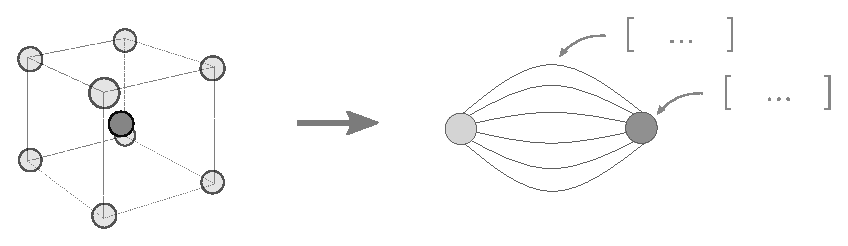
\includegraphics[scale=0.7]{crystalgraph.pdf}\pause
\end{center}

with atomic features associated with nodes and geometric features associated with edges

\end{frame}

\begin{frame}{Crystal Graphs cont. I}

Edges can be determined simply by distance cutoff (4 Ang.) and/or maximum number of neighbors for each node (12)

\begin{center}
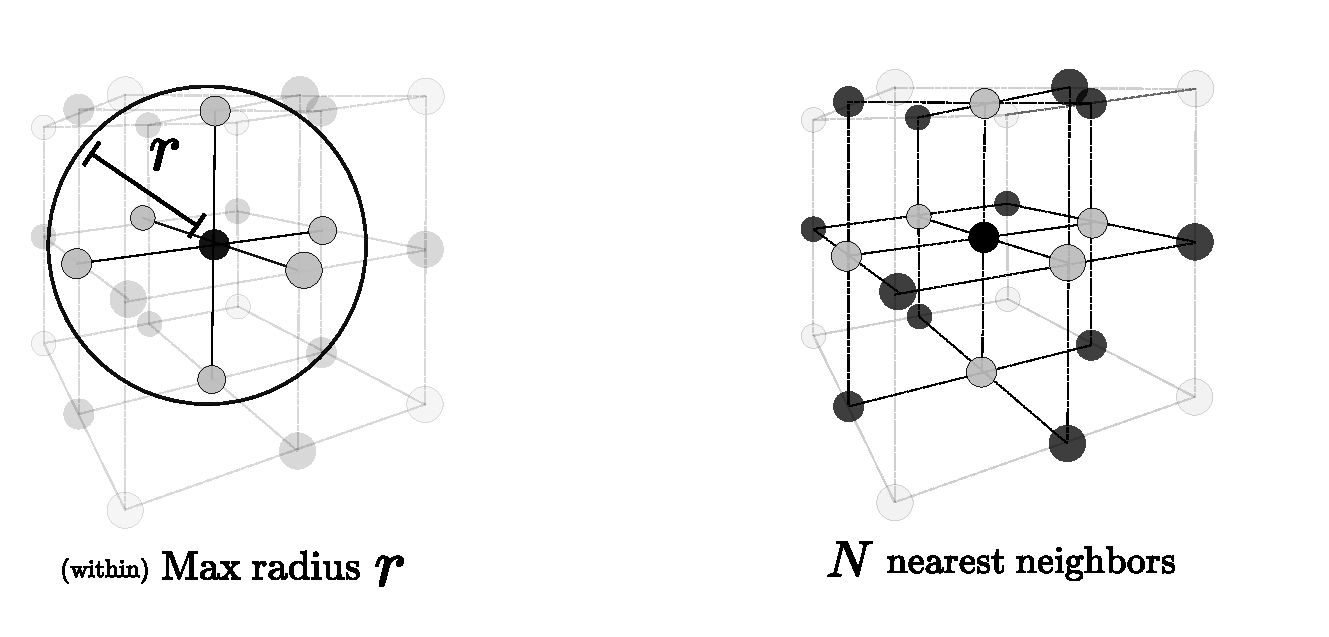
\includegraphics[scale=0.45]{ex_bondcriteria.pdf}
\end{center}
\end{frame}

\begin{frame}{Crystal Graphs cont. II}
Edge attributes then are constructed as a Gaussian expansion of interatomic distance:

\begin{center}
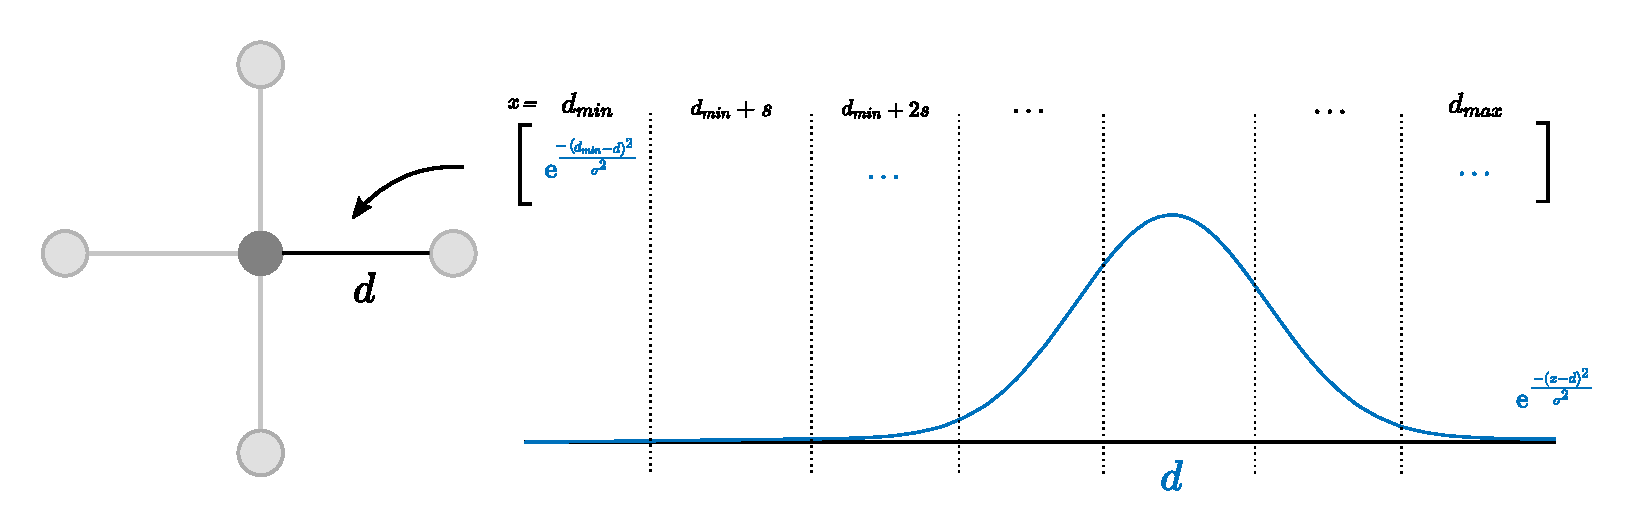
\includegraphics[scale=0.33]{bond_feat.pdf}
\end{center}
\end{frame}

\begin{frame}{Message Passing on Graphs}
Now, we need to update these features through some trainable function that acts on graph representations.


\medskip\pause

This is most generally accomplished by a message passing network applied to graph representations.\pause
\begin{gather*}
m_i^{t+1}=\sum_{n_j\in \mathcal{N}(i)} M_t(n_i^{t},e_{ij},n_j^t )\\
\\ 
n_i^{t+1}=U_t(n_i^t,m_i^{t+1})\\
\end{gather*}
Here, each node $n$ from layer $t$ to $t+1$ is updated according to an update function $U$, which takes as input messages formed from each pair of nodes containing the node to be updated.
\end{frame}

\begin{frame}{Graph Limitations}
Problem: \pause Our underlying representation encodes only distances between atoms!\pause

\begin{center}

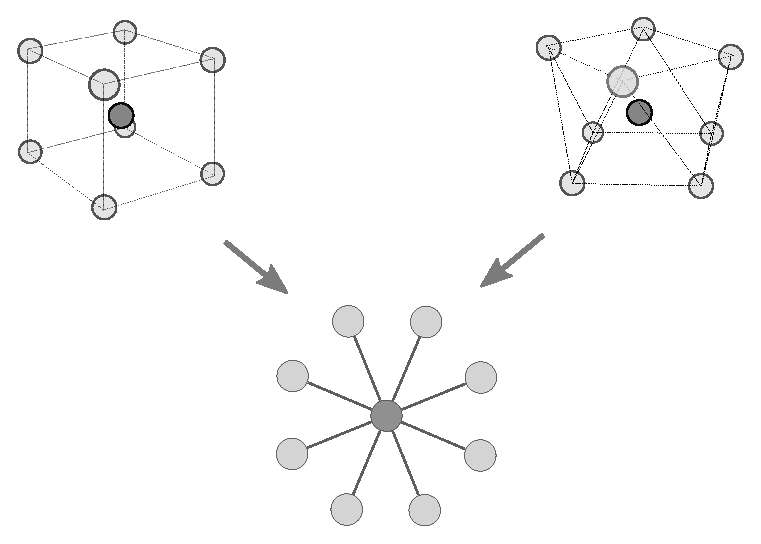
\includegraphics[scale=0.7]{crystalgraph_cntex.pdf}

\end{center}

So, as a rough example, the above two crystalline structures would have the same representations!
\end{frame} 

\section{Crystal Hypergraphs}
\begin{frame}{Solution: Hypergraphs!}
Hypergraphs allow us to have edges containing more than (or less than) two nodes.\pause 

\vspace{.5cm}

\begin{center}
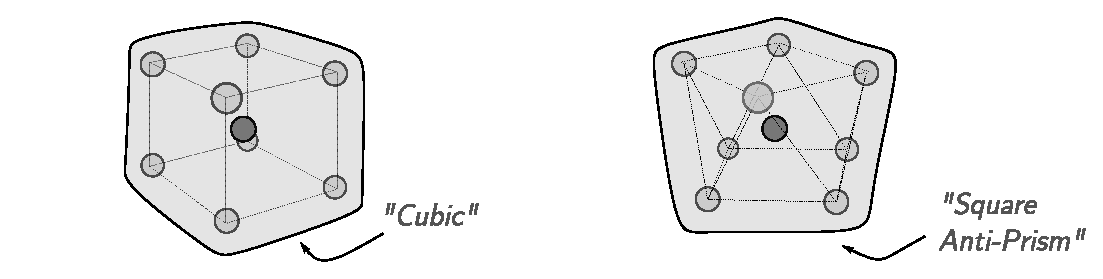
\includegraphics[scale=0.52]{crystalgraph_cntex_3.pdf}
\end{center}

\vspace{.5cm}

So, in a crystal hypergraph, we may define edges that explicitly describe this higher-order local geometry.
\end{frame}

\begin{frame}{Crystal Hypergraphs}

Hypergraphs give us a natural way to encode features with higher order physical structure, where hypergraph nodes still represent atoms of the underlying crystal structure.\pause
\begin{center}
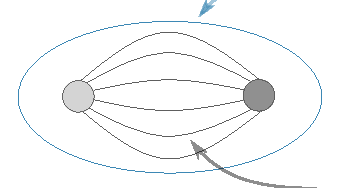
\includegraphics[scale=0.7]{hyperedge_ex.pdf}
\end{center}
\vspace{.5cm}

In a crystal hypegraph, we treat all different order structures (bonds, triplets, motifs, cells) in crystals on equal footing: \pause each has a corresponding hyperedge type with a certain set of features (distance, angle, order parameters, point group).
\end{frame}

\begin{frame}{Triplets as Hyperedges}
\small
Many modern models utilize 'triplet' information, specifically the angle between bonds, as the edge feature in a derived 'line-graph' in which nodes represent edges and edges represent overlapping bonds.

\begin{center}

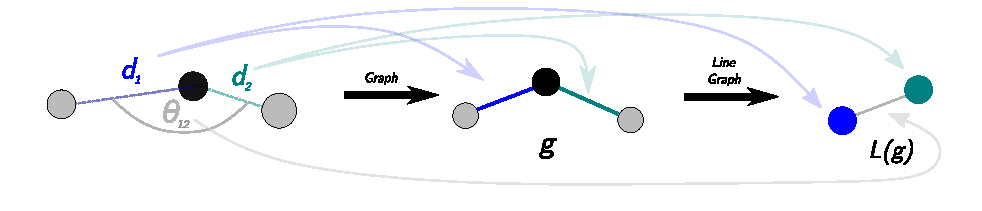
\includegraphics[scale=0.55]{line_graph_ex.pdf}

\end{center}\pause

This may be thought of more simply in terms of hyperedges of order three, formed again from overlapping bonds. The hyperedge features then are the angle formed between the bonds. \pause

\begin{center}

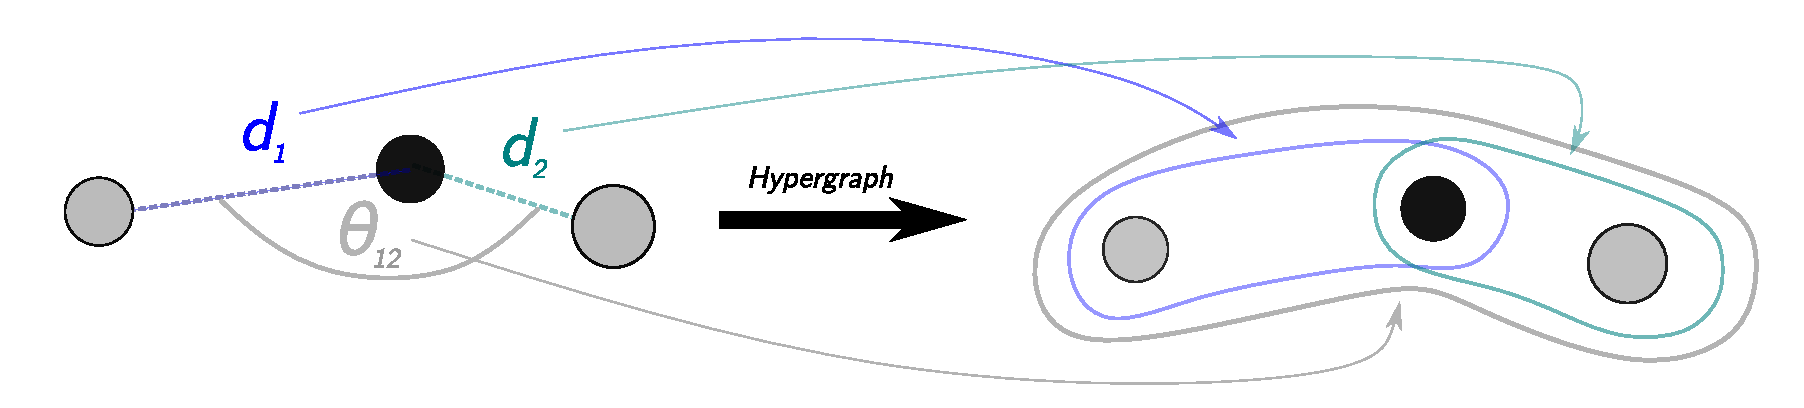
\includegraphics[scale=0.3]{triplet_ex.pdf}

\end{center}

\end{frame}

\begin{frame}{Local Environments as Hyperedges}
\small

Returning to our previous problem, how may we more simply  incorporate the missing local geometrical information?

\medskip\pause

We encode this lost geometrical information in larger hyperedges:

\medskip

\hspace{1cm}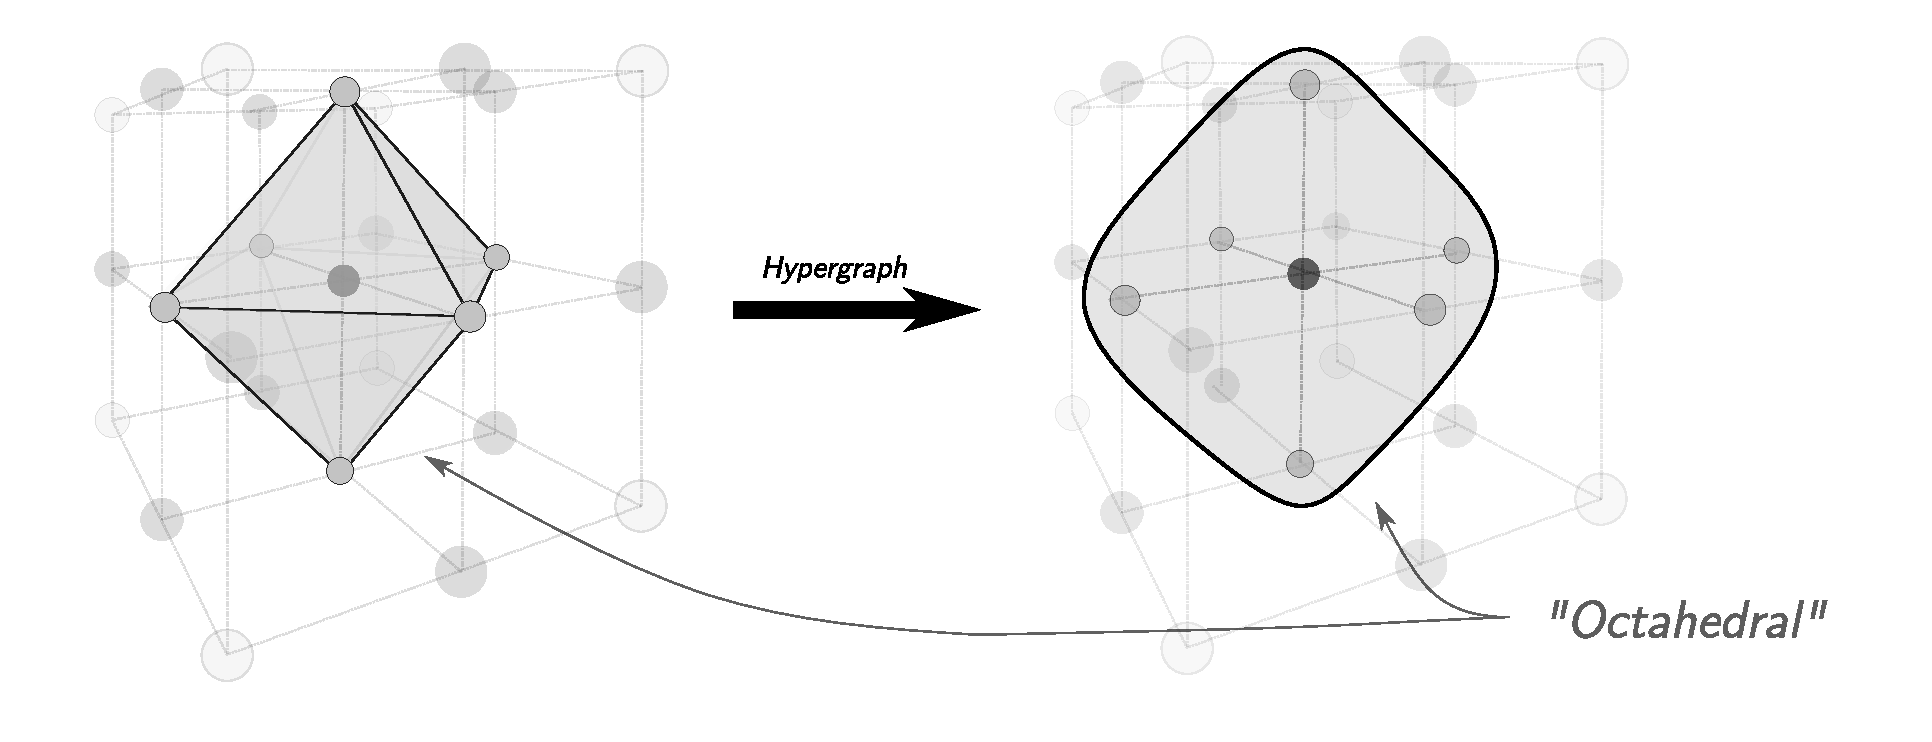
\includegraphics[scale=0.27]{motif_level_ex.pdf}

\medskip\pause

Where these hyperedges (of variable order, but generally $>1$) contain the entire first shell of neighbors. \pause 
The relevant geometrical information can then be encoded quantitatively with continuous symmetry measures, local structure order parameters, etc.
\end{frame}

%\begin{frame}{Determining Local Environments}
%To define a local environment, we need a way to systematically determine this environment for the relevant center sites.

%The determination of coordination environments often relies on the minimum distance between nearest neighbors for a site; and the largest solid angle spanned by a neighbors face in a Voronoi tesselation of the structure.
%\end{frame}

\begin{frame}{Cell Hyperedges}
\small
Another order of hyperedge we may consider is that describing the entire unit cell of some crystalline structure. \pause
\begin{center}
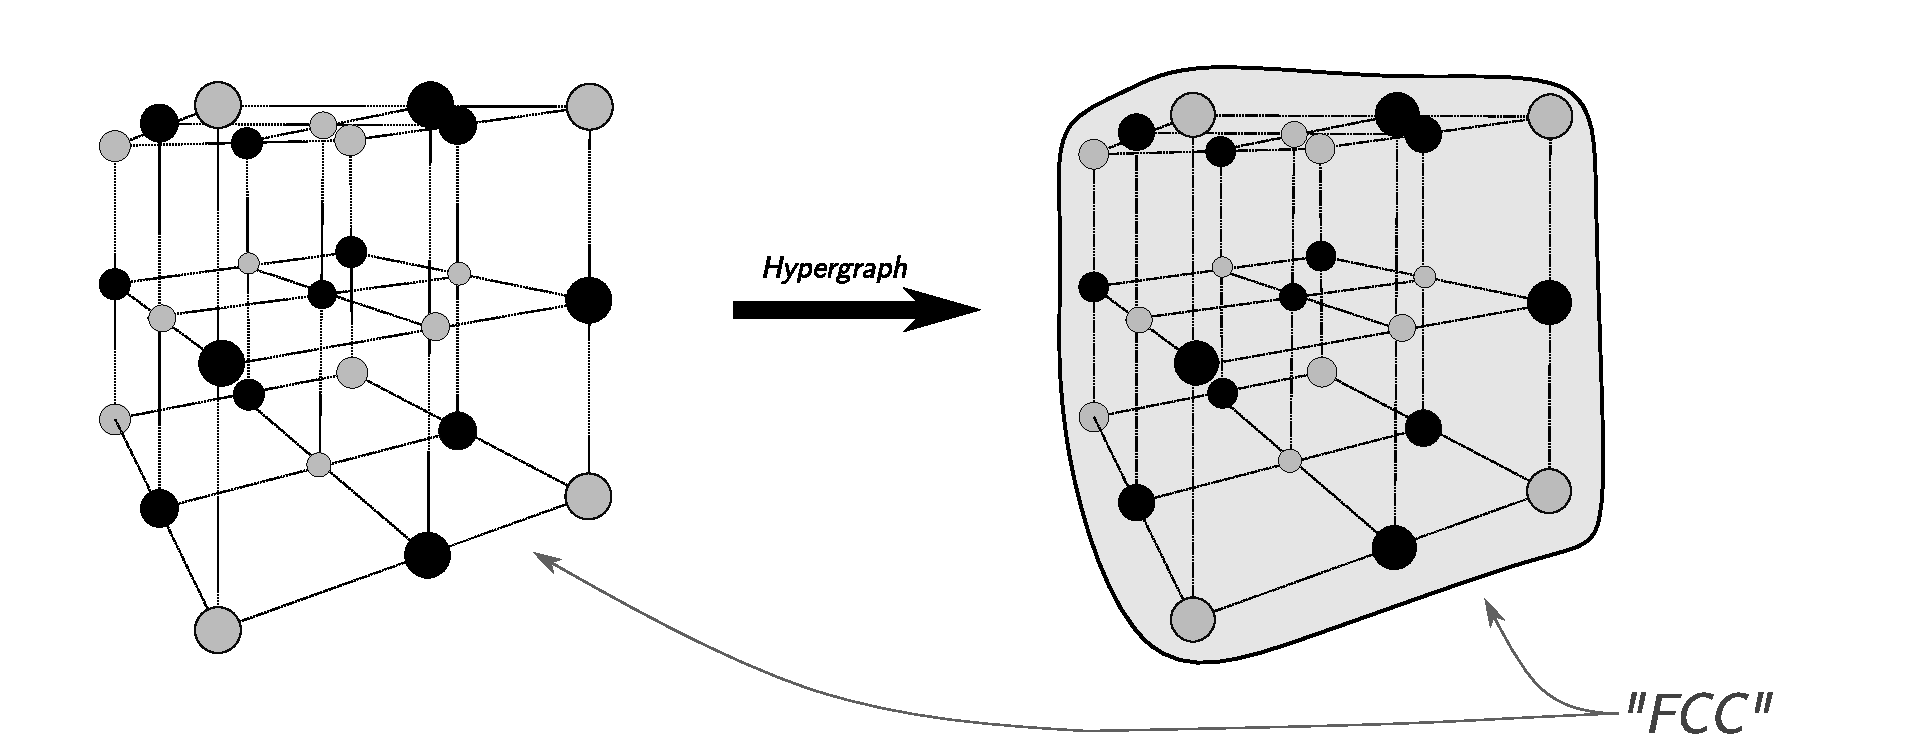
\includegraphics[scale=0.27]{cell_level_ex.pdf}
\end{center}\pause
These 'unit' cell hyperedges allow for the explicit inclusion of global crystalline structure properties, i.e. point group information.

\medskip\pause

This unit cell feature also may be learned through convolution and potentially used as a dynamic state vector.
\end{frame}

%\begin{frame}{Unit Cells as Hyperedges}
%Another order of hyperedge one may consider is that %describing the entire unit cell of some crystalline %structure. 

%A natural feature to encode in this cell-sized hyperedge is the point group of the system. 
%\end{frame}

\begin{frame}{Extending Message Passing to Hypergraphs}

Now, we need a suitable convolutional structure that applies to hypergraphs...\pause

\medskip

In the case of a hypergraph, the neighborhood of nodes relevant to each message are now a set (instead of the single neighboring node feature of classic MPNNs)\pause

\begin{gather*}
m_i^{t+1}=\sum_{h_j\ni x_i} M_t(n_i^{t},\underbrace{h_j^{t},\lbrace  n_w^t \vert n_w \in h_j }_{e_{ij},n_j}\rbrace)\\
\\
n_i^{t+1}=U_t(n_i^t,m_i^{t+1})\\
\end{gather*}

\pause
Furthermore, we may want to update nodes AND hyperedge features with different convolutional functions for different hyperedge types.
\end{frame}

\begin{frame}{Three Approaches to Hypergraph Convolution}
Three different approaches to message forming for hypergraphs were tested, each applicable to the updating of both node features and hyperedge features.\pause

\medskip

\textbf{1.} Naive Relatives Graph Convolution: This approach constructs a graph from the hypergraph
$$
n_i' =  n_i + f(n_i \oplus m_j ) 
$$

\medskip\pause

\textbf{2.} Interorder Hypergraph Convolution: This approach constructed a message for each node in each hyperedge (per origin node). It results in a generalization of message passing that exactly reproduces the latter in the case of only edges (of order 2, bonds)
$$
n_i' =  n_i + \sum_{n_k \in m_j}f(n_i \oplus m_j\oplus n_k ) 
$$
\end{frame}

\begin{frame}{Three Approaches cont.}

\textbf{3.} Hyperedge Aggregating Convolution: This approach constructs one message for each hyperedge (per origin node)
$$
n_i' =  n_i + f(n_i \oplus m_j\oplus \text{AGG}\lbrace n_k\in m_j \rbrace ) 
$$
\end{frame}



\begin{frame}{1. Relatives Graph Convolution}
The first approach, and perhaps the simplest, converts the initial hypergraph into a heterogeneous graph in which nodes represent hyperedges. \pause 

\begin{center}
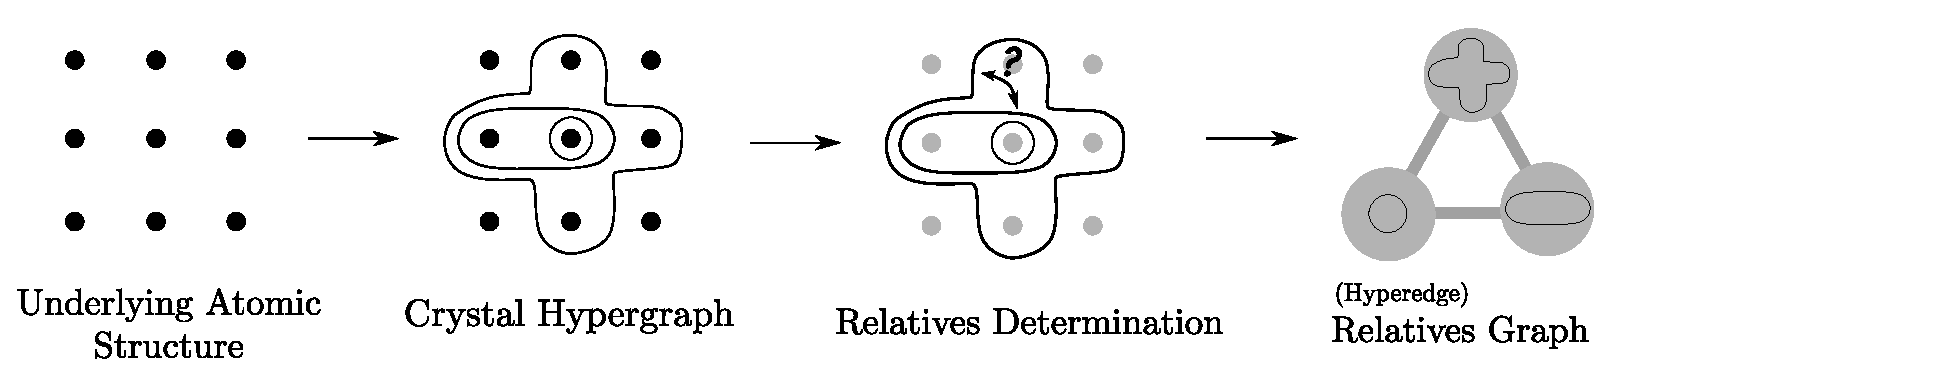
\includegraphics[scale=0.37]{relgraph_workflow_horiz.pdf}
\end{center}

This is essentially a line graph for hyperedges. \pause

Regular graph convolution may then be applied to this hyperedge 'relatives' graph, via it's \textit{edge index} (representing connections between hyperedge 'nodes'), resulting in node updates of the form below:
$$
x_i \rightarrow x_i + f_m(x_i\oplus m_j)
$$
\end{frame}

\begin{frame}{1. Relatives Graph Convolution cont.}
This approach has the benefit of working out-of-the-box with most current convolutional structures, but suffers in performance from a lack of neighbor features in it's form of messages.

\vspace{1cm}\pause

Note also that the number of messages here scales as $\mathcal{O}(nm)$, with $n$ the number of hyperedges and $m$ the average number of nodes in hyperedges. \pause This is similar to the scaling of a typical MPNN.
\end{frame}

\begin{frame}{2. Interorder Hypergraph Convolution}
The second approach utilizes just the hypergraph, defined by way of \textit{hyperedge-relations indices}:
\begin{align*}
[&[\text{origin-node-index},...],\\
&[\text{connecting-hyperedge-index},...],\\
&[\text{destination-node-index},...]]
\end{align*}

\medskip\pause

From these indices, messages may be read off in complete analogy to the usual graph case:
$$
x_i \rightarrow x_i + \sum_{x_k \in m_j} f_m(x_i\oplus m_j\oplus x_k)
$$\pause
This approach is nice in that it completely generalizing the usual message passing framework, but the number of messages scales as $\mathcal{O}(nm^2)$.

\end{frame}

\begin{frame}{3. Hyperedge Aggregation}
To deal with the variable sized neighborhoods of features, we may also simply aggregate the neighborhood features in the message passing phase\pause . Then, we essentially have the following form of convolution:
\begin{align*}
x_i \rightarrow x_i + f_m(x_i\oplus m_{j} \oplus \text{AGG}(\lbrace  n_w \vert n_w \in m_j \rbrace))
\end{align*}
This requires only that we define a \textit{hyperedge index} of dimension 2:
\begin{align*}
[&[\text{node-index},...],\\
&[\text{hyperedge-index},...]]
\end{align*}\pause
This also has the advantage that messages only scale as $\mathcal{O}(nm)$; as well as that, after aggregation, most existing graph convolutional structures may be applied.
\end{frame}

\section{Results}
\begin{frame}{Comparative Performance Testing}


The hyperedge aggregation method seems to be the best balance in terms of performance and computational cost.

\vspace{1cm}\pause

As a proof of concept, we implement a basic convolutional structure amenable to the hyperedge aggregation scheme (\textbf{3}) above, and compare performance between different sets of hyperedges.

\vspace{1cm}\pause

Here, we focus on performance between models with bond hyperedges and motif hyperedges.
\end{frame}

\begin{frame}{Hyperparameters and Model Architecture}
For each convolutional structure, testing was done for a model with 3 convolutional layers, an initial learning rate of 0.01, hidden node features of dimension 64, and a hidden output layer of dimension 128 (Similar to CGCNN's architecture). The loss function utilized is MSE.

\medskip\pause

Datasets are split 80\% for training and 20\% for validation tests. 

\end{frame}


\begin{frame}{(Materials-Project) Formation Energy}\small
Below, validation MAE is shown through training for formation energy. The total dataset includes 152,605 materials.
\begin{center}

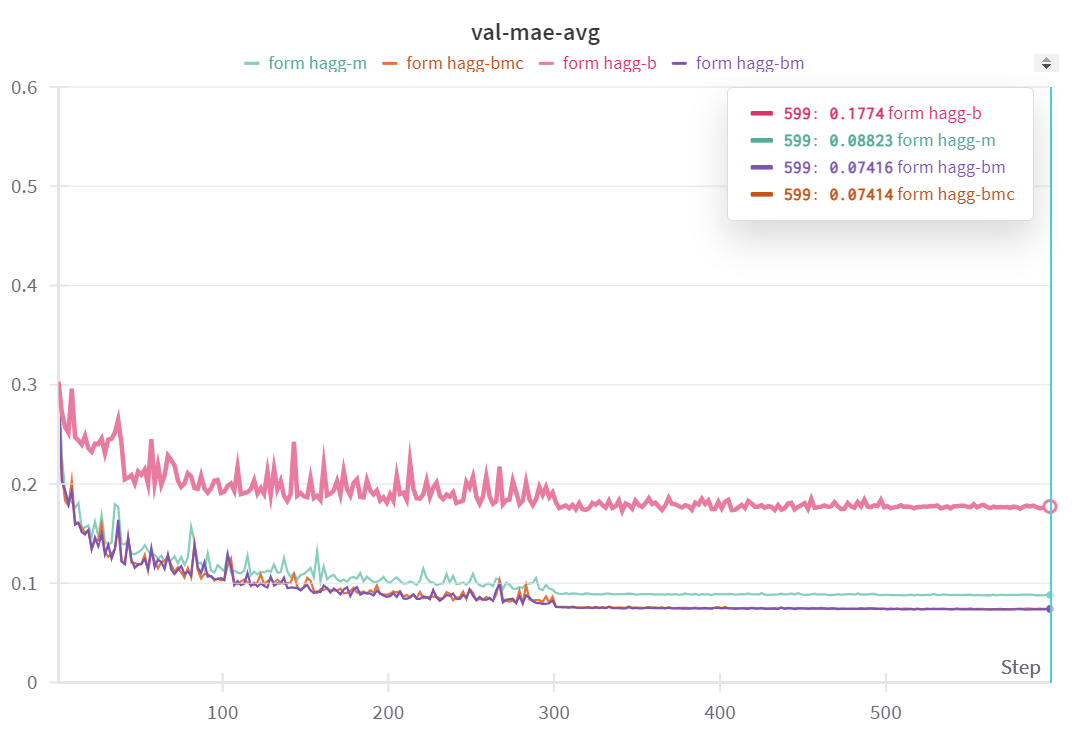
\includegraphics[scale=0.4]{formation_energy.png}

\medskip

\medskip


\begin{tabular}{c|ccc}
Model & Best MAE (eV/Atom) \\
\hline
Bond-only & 0.177 \\
Motif-only &  0.088\\
Bond \& Motif &  0.074\\
\end{tabular}
\end{center}
\end{frame}
\begin{frame}{(Materials-Project) Band Gap}
Below are results for band gap training, based on a dataset including 152,605 materials.
\begin{center}\small
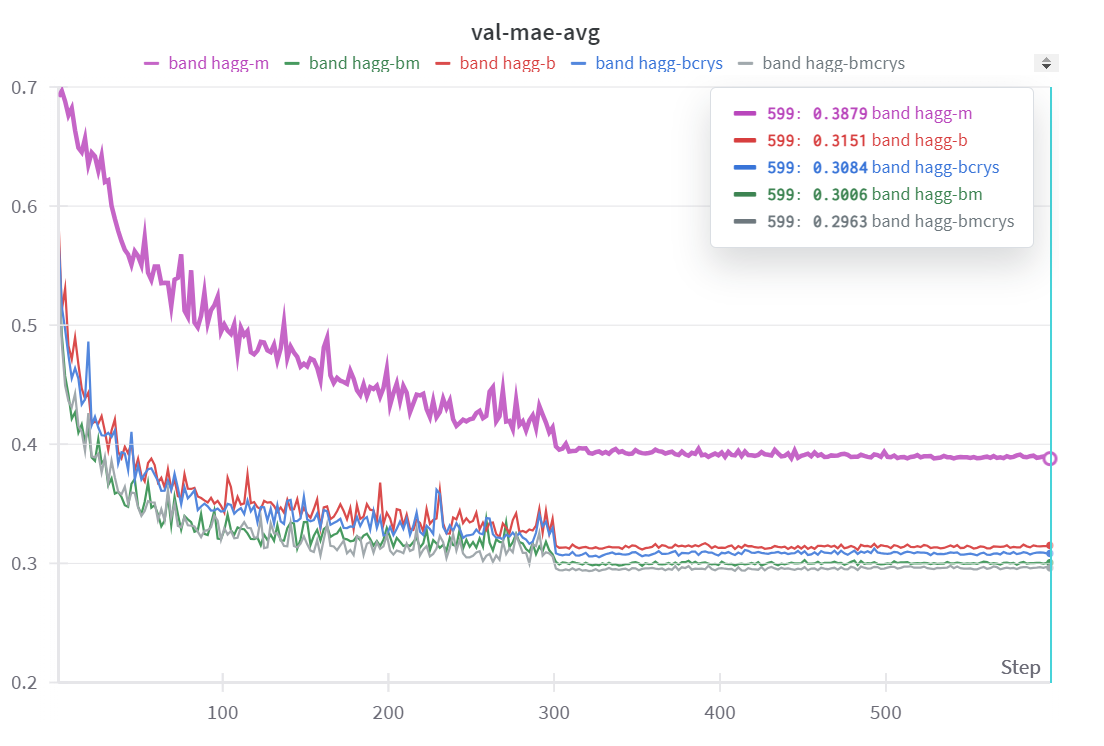
\includegraphics[scale=0.4]{band_gap.png}

\medskip

\begin{tabular}{c|ccc}
Model & Best MAE (eV) & w/ Crystal Feature \\
\hline
Bond-only & 0.315 & 0.3084 \\
Motif-only & 0.387 & \\
Bond \& Motif & 0.301 & 0.2963\\
\end{tabular}
\end{center}
\end{frame}
\begin{frame}{(Materials-Project) Metal/Non-metal}
Below, we test metal/non-metal classification for 152,605 materials.
\begin{center}
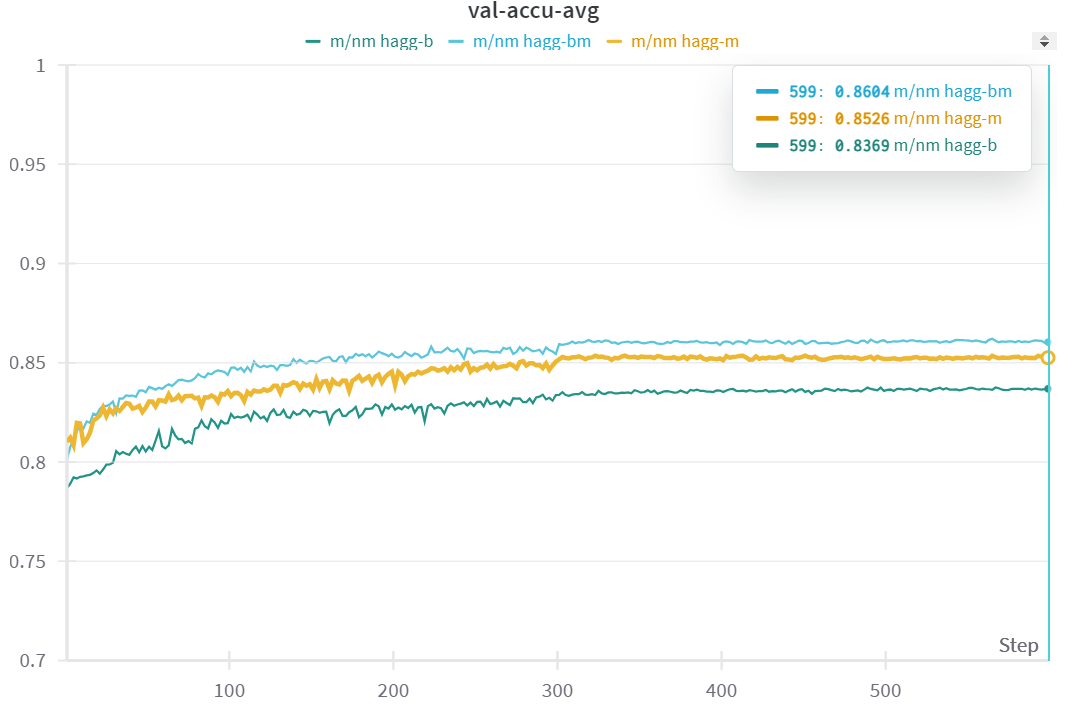
\includegraphics[scale=0.4]{metal_nonmetal.png}

\medskip



\begin{tabular}{c|ccc}
Model & Best Accuracy  \\
\hline
Bond-only & .837\\
Motif-only & .853\\
Bond \& Motif & .860\\
\end{tabular}
\end{center}
\end{frame}

\begin{frame}{(MatBench) Perovskites}\small
Below, we test on 18,928 calculated formation energies for Perovskites.
\begin{center}
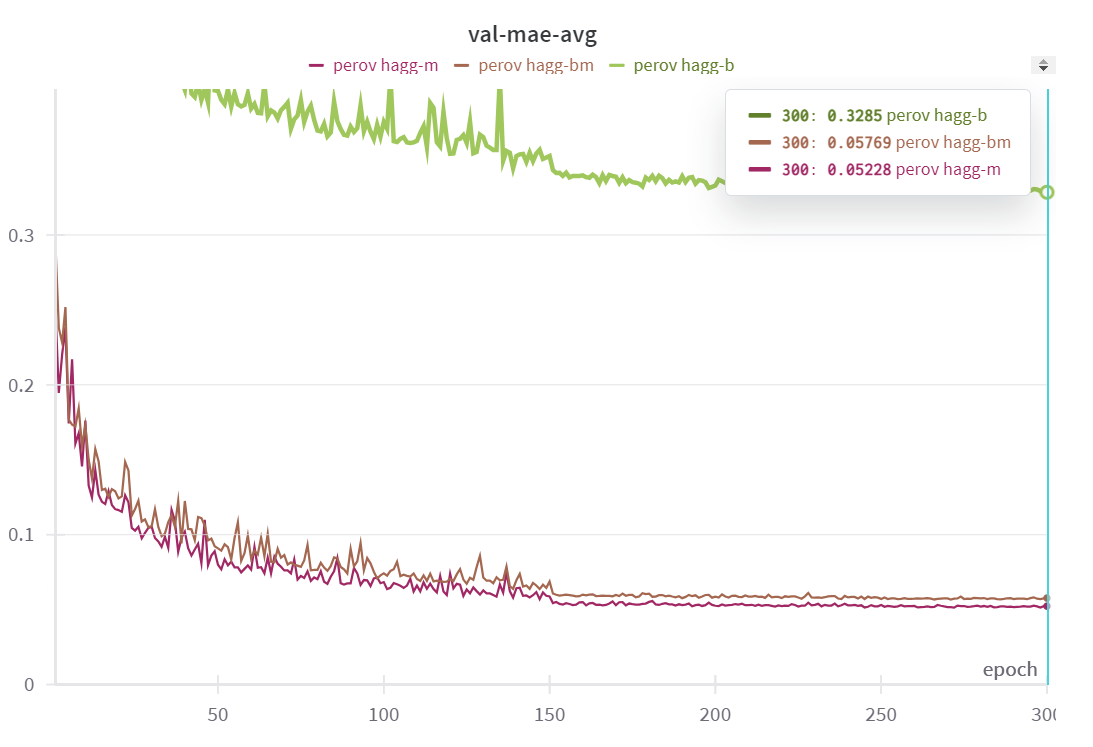
\includegraphics[scale=0.4]{perovskites.png}

\medskip


\begin{tabular}{c|ccc}
Model & Best MAE (eV/Atom) \\
\hline
Bond-only & 0.329\\
Motif-only & 0.052\\
Bond \& Motif & 0.058\\
\end{tabular}
\end{center}
\end{frame}
\begin{frame}{(MatBench) Phonons}\small

Below, we test on a dataset of 1,265 materials with the target being the highest calculated frequency optical phonon mode peak.
\begin{center}

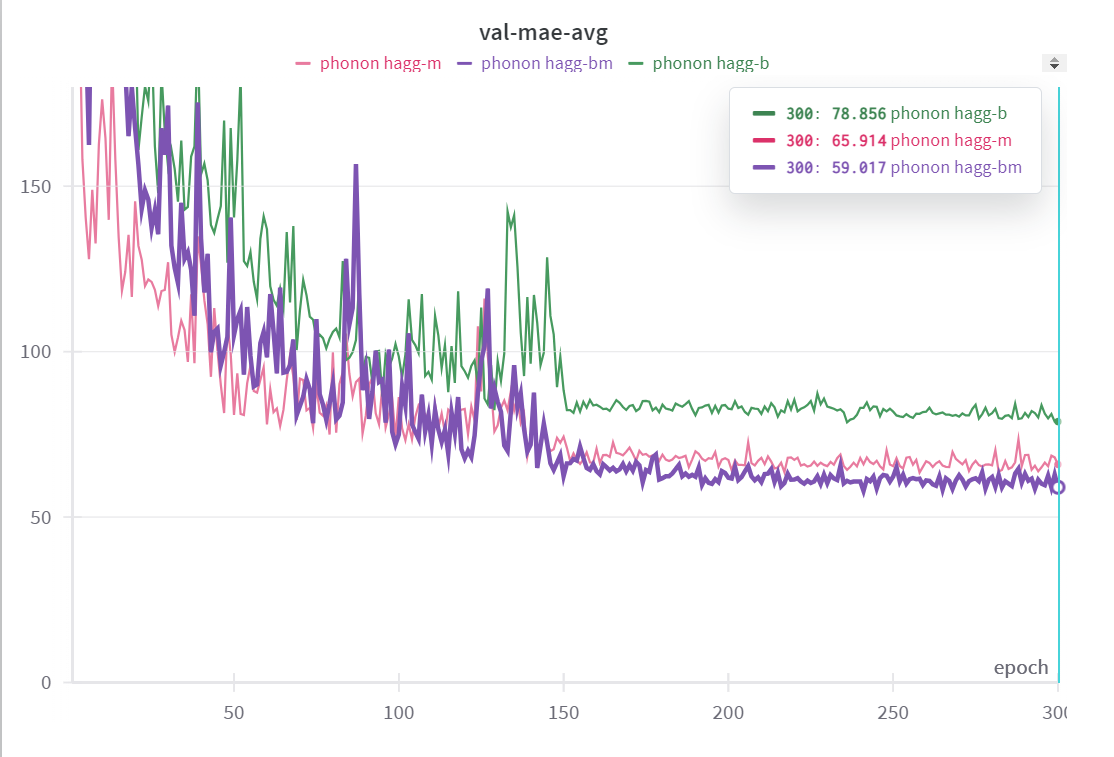
\includegraphics[scale=0.4]{phonons.png}

\medskip

\begin{tabular}{c|ccc}
Model & Best MAE (cm$^{-1}$) \\
\hline
Bond-only & 78.9\\
Motif-only & 65.9\\
Bond \& Motif & 59.0\\
\end{tabular}
\end{center}
\end{frame}
\begin{frame}{(MatBench) Shear Moduli $\log_{10}(G_{vrh})$}
\small
Below, we test on the calculated shear moduli of 10,987 materials
\begin{center}


\begin{tabular}{c|ccc}
Model & Best MAE (eV) \\
\hline
Bond-only & \\
Motif-only & \\
Bond \& Motif & \\
\end{tabular}
\end{center}
\end{frame}
\begin{frame}{(MatBench) Dielectrics}\small
Below, we test on the calculated refractive index of 4,764 materials
\begin{center}
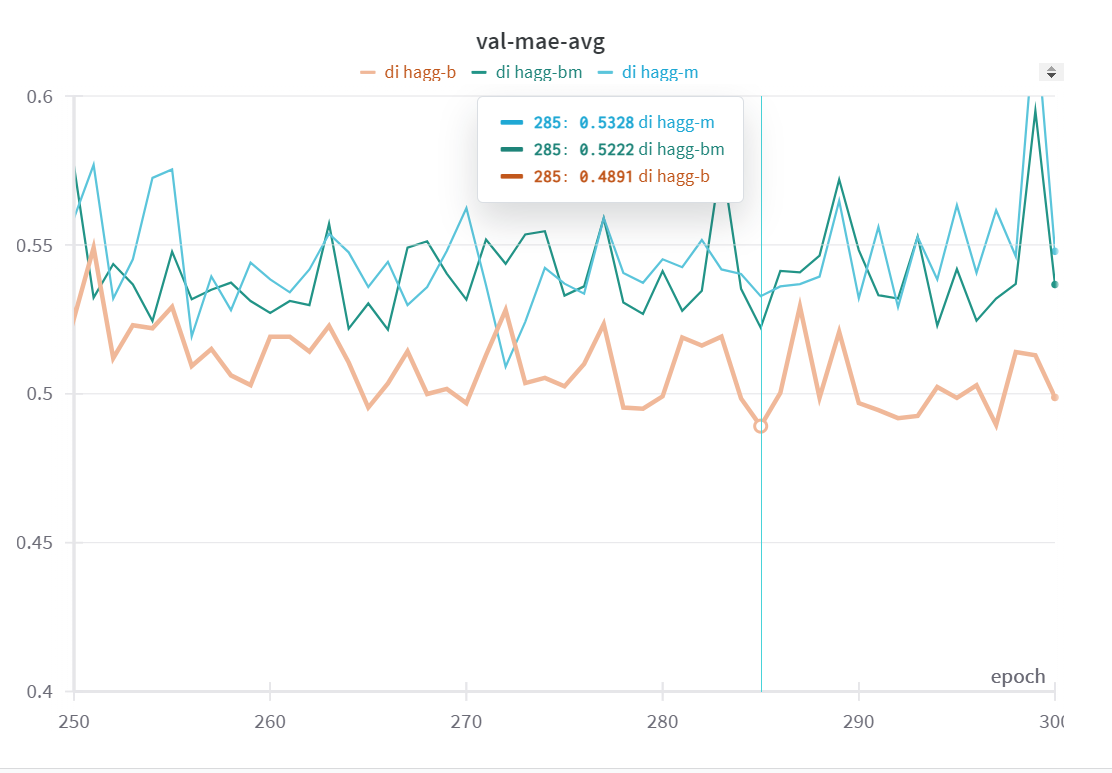
\includegraphics[scale=0.43]{dielectric.png}

\medskip

\medskip
\begin{tabular}{c|ccc}
Model & Best MAE \\
\hline
Bond-only & .4891\\
Motif-only & .5328\\
Bond \& Motif & .5222\\
\end{tabular}
\end{center}
\end{frame}

\begin{frame}{Overview of Experimental Results}\small

$\bullet$  Electronic tasks (band gap, dielectric targets) seem to benefit much less, or be negatively impacted, by this additional information. \pause It seems pair-wise correlators are, in general, a better descriptor for such tasks.

\vspace{.5cm}\pause

$\bullet$ Formation energy tasks benefit greatly from included motif (i.e. higher order geometrical) descriptors

\vspace{.5cm}\pause

$\bullet$ In the case of Perovskites (a harder set of formation energy targets), this geometrical information seems even more impactful\pause . Though, it also may just help more for the smaller dataset available for training.

\vspace{.5cm}\pause

$\bullet$ Phonons (also heavily dependent on geometrical information) seem to also benefit greatly from motif-level features

\vspace{.5cm}

\end{frame}

\begin{frame}{GUESS}

Elastic properties (bulk, shear moduli) should also benefit more from motif information than bond information, since these are also related to overall structure.
\end{frame}

\begin{frame}{Conclusion}
$\bullet$ Graphs are limited in their expression of higher-order (above pair-wise) features of crystal structures

\vspace{.5cm}\pause

$\bullet$ Crystal hypergraphs give us a natural way to encode different types of features in one representation
\end{frame}
\end{document}